\documentclass[aspectratio=169]{beamer}

\usepackage{mhasbiarz}
\graphicspath{{./Images}}

%newtheorem
\newtheorem{teorema}{Teorema}[section]
\newcommand{\lcm}{\operatorname{lcm}}
\renewcommand{\theteorema}{\arabic{section}.\arabic{teorema}}
\newtheorem{sifat}[teorema]{Sifat}
\newtheorem{akibat}[teorema]{Akibat}
\newtheorem{proposisi}[teorema]{Proposisi}
\newtheorem{definisi}[teorema]{Definisi}

%Block Baru
\newenvironment{variableblock}[3]{%
	\setbeamercolor{block body}{#2}
	\setbeamercolor{block title}{#3}
	\begin{block}{#1}}{\end{block}}

\newenvironment{rbox}[1]{
	\setbeamercolor{block body}{bg=mygreen!4,fg=black}
	\setbeamercolor{block title}{bg=mygreen!90,fg=white}
	\begin{block}{#1}}{\end{block}}


\begin{document}
\title{\color{mygreen} Riset Operasi B}
\subtitle{\color{mygreen!90} Kelompok 4}

\author[mhasbiarz]{\color{black}
Ridho Maulana Asrofi \\
Aprila Adzkiyan Najah \\
Nala Kirana Prastiwi \\
Delia Noor Mavianti \\
Moh Hasbi Alfarizi }

\date{{\footnotesize \color{mygreen!90}} }

\subject{}
\titlegraphic{\begin{tikzpicture}[overlay, remember picture]
		\node[xshift=5cm,yshift=-8.02cm]{
\includegraphics[width=12cm]{img1}
		};
	\end{tikzpicture}
	\begin{tikzpicture}[overlay, remember picture]
		\node[xshift=11cm,yshift=-4mm]{
\includegraphics[width=5cm]{logo}
		};
	\end{tikzpicture}
}

\maketitle

\begin{frame}
    \begin{center}
    \color{mygreen} \huge \textbf{On the Application of the Open Jackson Queuing Network in Hospital}
    \end{center}
    \begin{center}
        Arum Helmi Manggala Putri, Irwan Endrayanto
    \end{center}
    \\
    \begin{center}
        \color{mygreen!90} \large Kelompok 4
    \end{center}
\end{frame}

\begin{frame}{Table of Contents}
	\tableofcontents
\end{frame}

\section{\color{mygreen}\huge Pendahuluan}
\begin{frame}{Pendahuluan}
Open Jackson queuing network adalah sistem antrian baris terbuka yang terdiri dari beberapa stasiun layanan. Pada open Jackson queuing network, pasien tiba dari luar sistem untuk mendapatkan layanan dan kemudian meninggalkan sistem. Teori open Jackson queuing network digunakan untuk menentukan model sistem antrian yang akan dibangun berdasarkan diagram tahap layanan di rumah sakit.
\end{frame}
    

\section{\color{mygreen}\huge Rumusan Masalah}
\begin{frame}{Rumusan Masalah}
\begin{itemize}
    \item Apakah yang dimaksud dengan open jackson queuing network?
    \item Bagaimana model open jackson queuing network dapat diterapkan untuk menentukan model sistem antrian layanan di rumah sakit dan bala nced equationsnya?
    %\item bagaimana metode Moore-Penrose pseudo-inverse dapat digunakan untuk menyelesaikan sistem persamaan linear yang dibentuk oleh model sistem antrian tersebut sehingga memungkinkan penghitungan ukuran kinerja seperti jumlah rata-rata pasien dan waktu tunggu pasien dalam kondisi steady-state?






\end{itemize}
\end{frame}


\section{\color{mygreen}\huge Studi Literatur}
\begin{frame}{Studi Literatur}
\begin{rbox}{Model Jaringan Antrian di Rumah Sakit}
\justifying Fenomena antrian dapat terjadi ketika permintaan suatu layanan melebihi kapasitas yang tersedia. Antrian pasien di rumah sakit untuk mendapatkan layanan medis menyebabkan pasien kehilangan waktu, tenaga, biaya, dan menurunnya tingkat kepercayaan pasien terhadap rumah sakit. Oleh karena itu, diperlukan teori antrian untuk memberikan gambaran atau model terkait permasalahan sistem antrian.  

Penelitian ini mengadopsi Open Jackson Queueing Network untuk memodelkan dan menganalisis sistem antrian yang ada dengan tujuan pasien mendapatkan rasa nyaman dan puas terhadap pelayanan yang diberikan.
\end{rbox}
\end{frame}
\begin{frame}{Studi Literatur}
\begin{rbox}{Open Jackson Queueing Network}
\justifying Open Jackson Queueing Network adalah jaringan yang terdiri dari $N$ stasiun dengan satu server. Proses kedatangan di luar stasiun $i$ dengan $i = 1,2,3,...,N$ berdistribusi Poisson dengan rate $\lambda_{0i} (\lambda \geq 0 \forall i)$. Setiap antrian memiliki layanann yang berdistribusi secara eksponensial dengan waktu layanan rata-rata $E[W_i]$.
\\
Pasien dipindahkan dari stasiun $i$ ke $j$ dengan probabilitas perpindahan statenya independen $p_{ij}$ $(0 \leq p_{ij} \leq 1)$. Parameter $p_{i0}$ menunjukkan sebagian kecil pasien yang meninggalkan jaringan dalam antrian $i$. Tingkat kedatangan $\lambda_j$ di stasiun $j$ diberikan oleh :
\begin{center}
    $\lambda_j = \lambda_{0j} + \sum \limits_{i=1}^{N} \lambda_i p_{ij},$ dengan $j= 1,2,3,...,N$
\end{center}   
\end{rbox}
\end{frame}
%\\
\begin{frame}
\begin{rbox}
    \justifying dan terdiri dari kedatangan ke  antrian $j$ dari luar dan di dalam jaringan.Jaringan antrian dengan karakteristik ini disebut Open Jackson Queueing Network. Di dalam teorema jackson, solusi bentuk produk untuk jaringan yang terdisi dari $N$ stasiun dengan satu server diberikan oleh :
    \begin{center}
        $P(n_1,...,n_N) = \prod\limits_{i=1}^N \rho_i^{n_i}(i-\rho_i)$,$n_i \geq 0$ , dengan $i=1,2,...,N$
    \end{center}
    Dimana $\rho = \frac{\lambda_i}{\mu_i}$ dan $p(n_i)$ adalah probabilitas $n$ pasien di stasiun $i$
\end{rbox}
    
\end{frame}

\begin{frame}{Studi Literatur}
\begin{rbox}{Analisis Antrian Satu Server M/M/1 : (FCFS/$\infty$/$\infty$)}
    Karakteristik dan asumsi dari model antrian di semua stasiun layanan dapat disimpulkan menjadi notasi Kendall $(M/M/1)$: (FCFS/$\infty$/$\infty$), \textcolor{blue}{waktu kedatangan dan waktu keberangkatan diasumsikan terdistribusi Poisson dan eksponensial}. Selain itu, sistem antrian di semua stasiun layanan hanya memiliki satu server dan kapasitas sumber panggilan yang tidak terbatas. %Gambar 1 adalah diagram yang menunjukkan model $(M/M/1)$: (FCFS/$\infty$/$\infty$).
    \begin{figure}
        \centering
        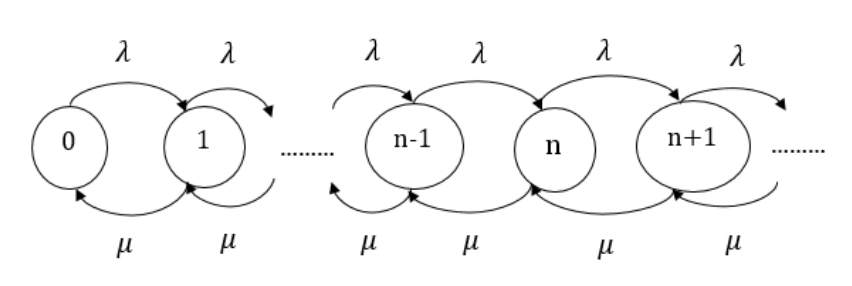
\includegraphics[width=0.52\linewidth]{mm1.PNG}
        \caption{Daigram Transisi State di Antrean M/M/1}
        \label{fig:enter-label1}
    \end{figure}
    
    %\begin{center}
       % 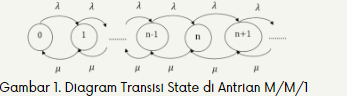
\includegraphics{Screenshot ppt rob.png}

   % \end{center}
\end{rbox}
\end{frame}

\begin{frame}{{Studi Literatur}}
\begin{rbox}{Analisis Antrian Satu Server M/M/1 : (FCFS/$\infty$/$\infty$)}
     Berdasarkan Gambar 1, sistem berada dalam keseimbangan statistik ketika tingkat kedatangan seimbang dengan tingkat keberangkatan di setiap state $n$ dengan $n$ = 1,2,3, ... . Keseimbangan statistik menghasilkan balance equation lokal dan dapat dinyatakan sebagai
    \begin{center}
    $P_1 = \frac{\lambda}{\mu}P_0$ 
    \end{center}
\end{rbox}
\end{frame}
    
\section{\color{mygreen}\huge Pembahasan}
\begin{frame}{Pembahasan}
    \begin{rbox}{Diagram Skematik Jaringan Antrean di Fasilitas Rumah Sakit}
        Jaringan antrean di rumah sakit ini terdiri dari beberapa ruangan layanan, di antaranya adalah \textcolor{red}{ruang registrasi}, \textcolor{red}{ruang pemeriksaan (oleh perawat)}, \textcolor{red}{ruang pemeriksaan (oleh dokter)}, dan \textcolor{red}{ruang administrasi serta farmasi}. Tingkat kedatangan pelanggan di setiap ruang layanan ditandai dengan $\lambda_i$ dan tingkat keberangkatan pelanggan ditandai dengan $\mu_i$ dengan $i = 1,2,3, . . . .$ Diagram skema jaringan di rumah sakit diberikan pada gambar sebagai berikut:    
    \end{rbox}
\end{frame}

\begin{frame}{Pembahasan}
        \centering
        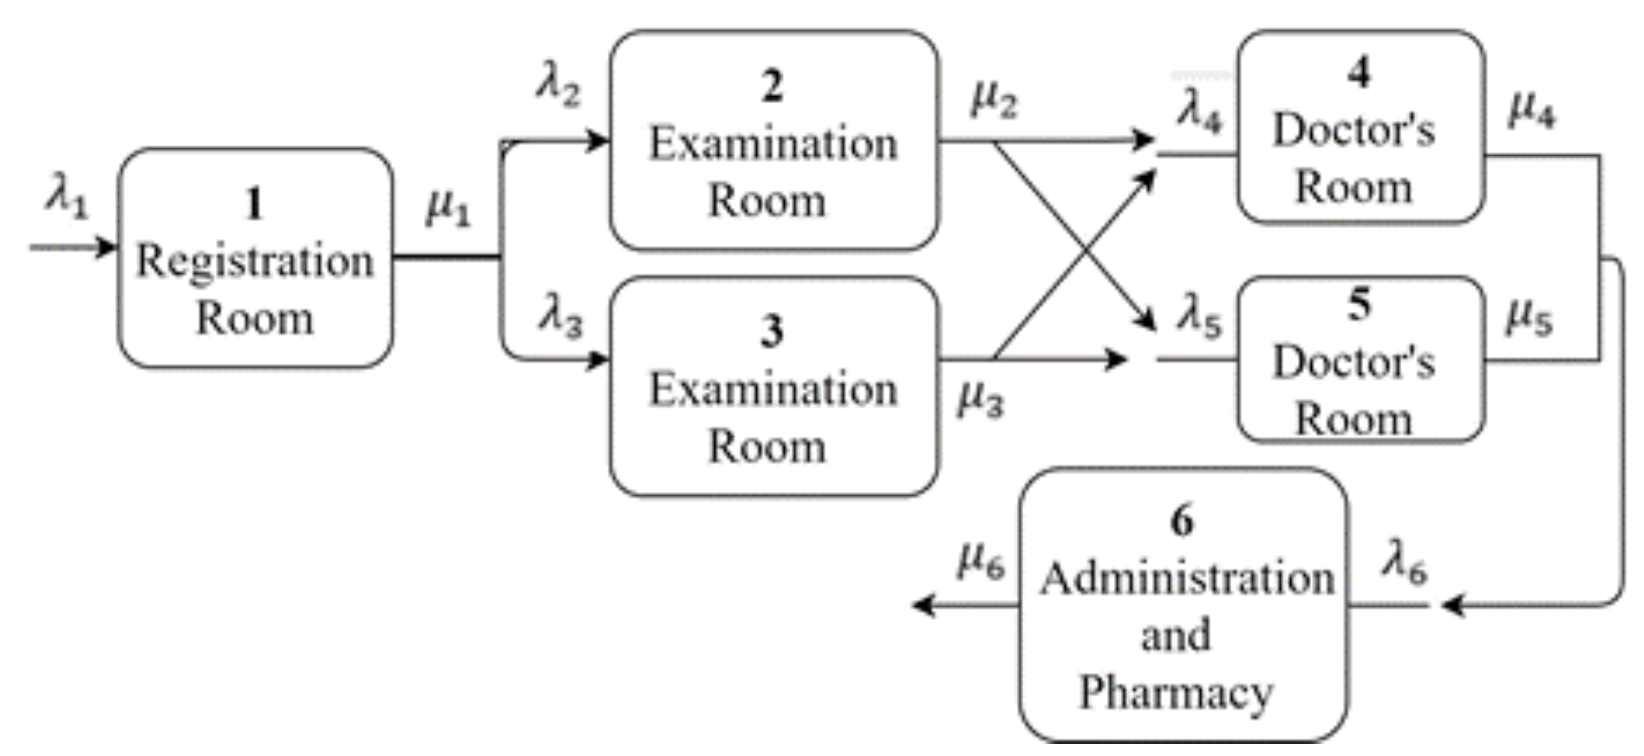
\includegraphics[width=0.6\linewidth]{Images/Diagram Skematik.png}
        
    \justifying Namun, untuk kasus jaringan seperti diagram diatas dalam perhitungannya terlalu kompleks, sehingga hanya diambil beberapa bagian saja agar perhitungannya lebih sederhana yang diberikan pada Gambar 2 sebagai berikut.

\end{frame}

\begin{frame}{Diagram}
Pasien yang datang harus melewati service unit 1 yaitu ruang registrasi selanjutnya pasien menuju ke service unit 2 dan 3. Tidak hanya itu, pasien di unit 3 bisa menuju ke unit 2 apabila memerlukan ke ruang dokter.
   \begin{figure}
        \centering
        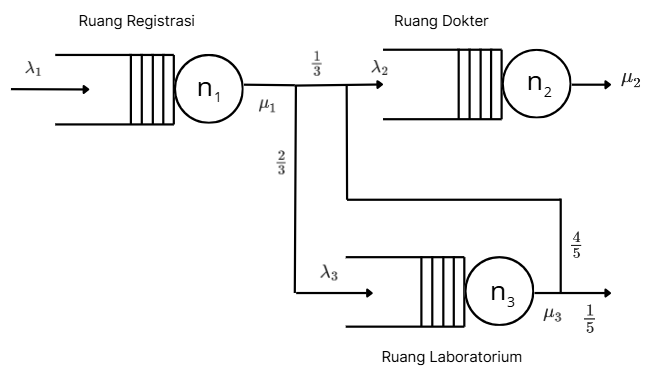
\includegraphics[width=0.55\linewidth]{Images/diagram 1.PNG}
        \caption{Diagram Skematik Jaringan Antrian Sederhana di Rumah sakit}
        \label{fig:enter-label1}
    \end{figure} 
\end{frame}
\begin{frame}{Pembahasan}
    \begin{rbox}{Jenis Model dan Asumsi}
    Jenis model antrean yang digunakan pada penelitian ini adalah model antrean \textbf{M/M/1} atau setiap \textit{server station} terdiri dari satu \textit{server} dengan laju kedatangan $(\lambda)$ dan keberangkatan $(\mu)$ pelanggan berdistribusi Poisson.\\ \\
    Adapun asumsi-asumsi yang digunakan pada penelitian ini yaitu:
    \begin{enumerate}
        \item [(1)] \textbf{\textit{No reneging}} atau pelanggan tidak meninggalkan antrian jika mereka telah menunggu terlalu lama untuk mendapatkan layanan.
        \item [(2)] \textbf{\textit{No Balking}} atau pelanggan tidak meninggalkan antrian jika mereka telah menunggu terlalu lama untuk mendapatkan layanan.
    \end{enumerate}
    \end{rbox}
\end{frame}

\begin{frame}{STATE SPACE}
  \begin{enumerate}
      \item Notasi $n_{1}(t)$ menyatakan banyaknya pasien yang sedang menunggu untuk dilayani oleh service unit 1 (ruang registrasi).
      \item Notasi $n_{2}(t)$ menyatakan banyaknya pasien yang sedang menunggu untuk dilayani oleh service unit 2 (ruang Dokter).
      \item  Notasi $n_{3}(t)$ menyatakan banyaknya pasien yang sedang menunggu untuk dilayani oleh service unit 3 (ruang laboratorium).
  \end{enumerate}  
\end{frame}

\begin{frame}{TRANSITION STATE}
Berikut merupakan transition state dari diagram antrian di rumah sakit : 
\begin{table}[h]
\centering
\begin{tabular}{|c|c|c|}
\hline
{\textbf{Dari} & \textbf{Menuju} & \textbf{Rate}} \\
\hline
($n_{1},n_{2},n_{3}$) & ($n_{1}+1,n_{2},n_{3}$) & $\lambda_{1}$ \\
($n_{1},n_{2},n_{3}$) & ($n_{1}-1,n_{2}+1,n_{3}$) & $\frac{1}{3}\mu_{1}$ \\
($n_{1},n_{2},n_{3}$) & ($n_{1}-1,n_{2},n_{3}+1$) & $\frac{2}{3}\mu_{1}$ \\
($n_{1},n_{2},n_{3}$) & ($n_{1},n_{2}-1,n_{3}$) & $\mu_{2}$ \\
($n_{1},n_{2},n_{3}$) & ($n_{1},n_{2},n_{3}-1$) & $\frac{1}{5}\mu_{3}$ \\
($n_{1},n_{2},n_{3}$) & ($n_{1},n_{2}+1,n_{3}-1$) & $\frac{4}{5}\mu_{3}$ \\
\hline
\end{tabular}
\caption{Tabel transition state}
\label{tab:contoh}
\end{table}
\end{frame}

\section{\color{mygreen}\huge Diagram Transition}
\begin{frame}{Diagram Transition}
    \begin{figure}
        \centering
        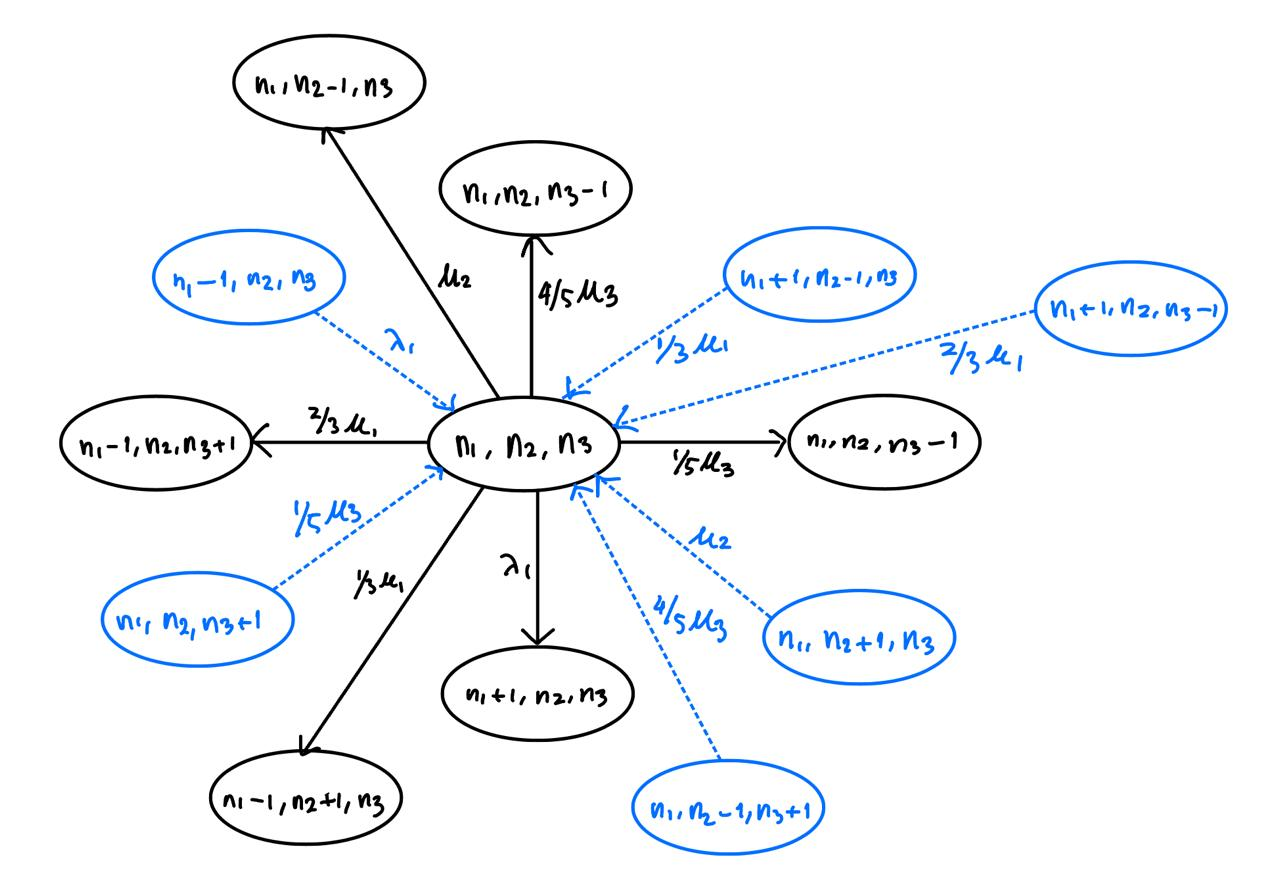
\includegraphics[width=0.65\linewidth]{n1,n2,n3.jpg}
        \caption{$n_1,n_2,n_3$}
        \label{fig:enter-label1}
    \end{figure}
\end{frame}

\begin{frame}{Diagram Transition}
    \begin{figure}
        \centering
        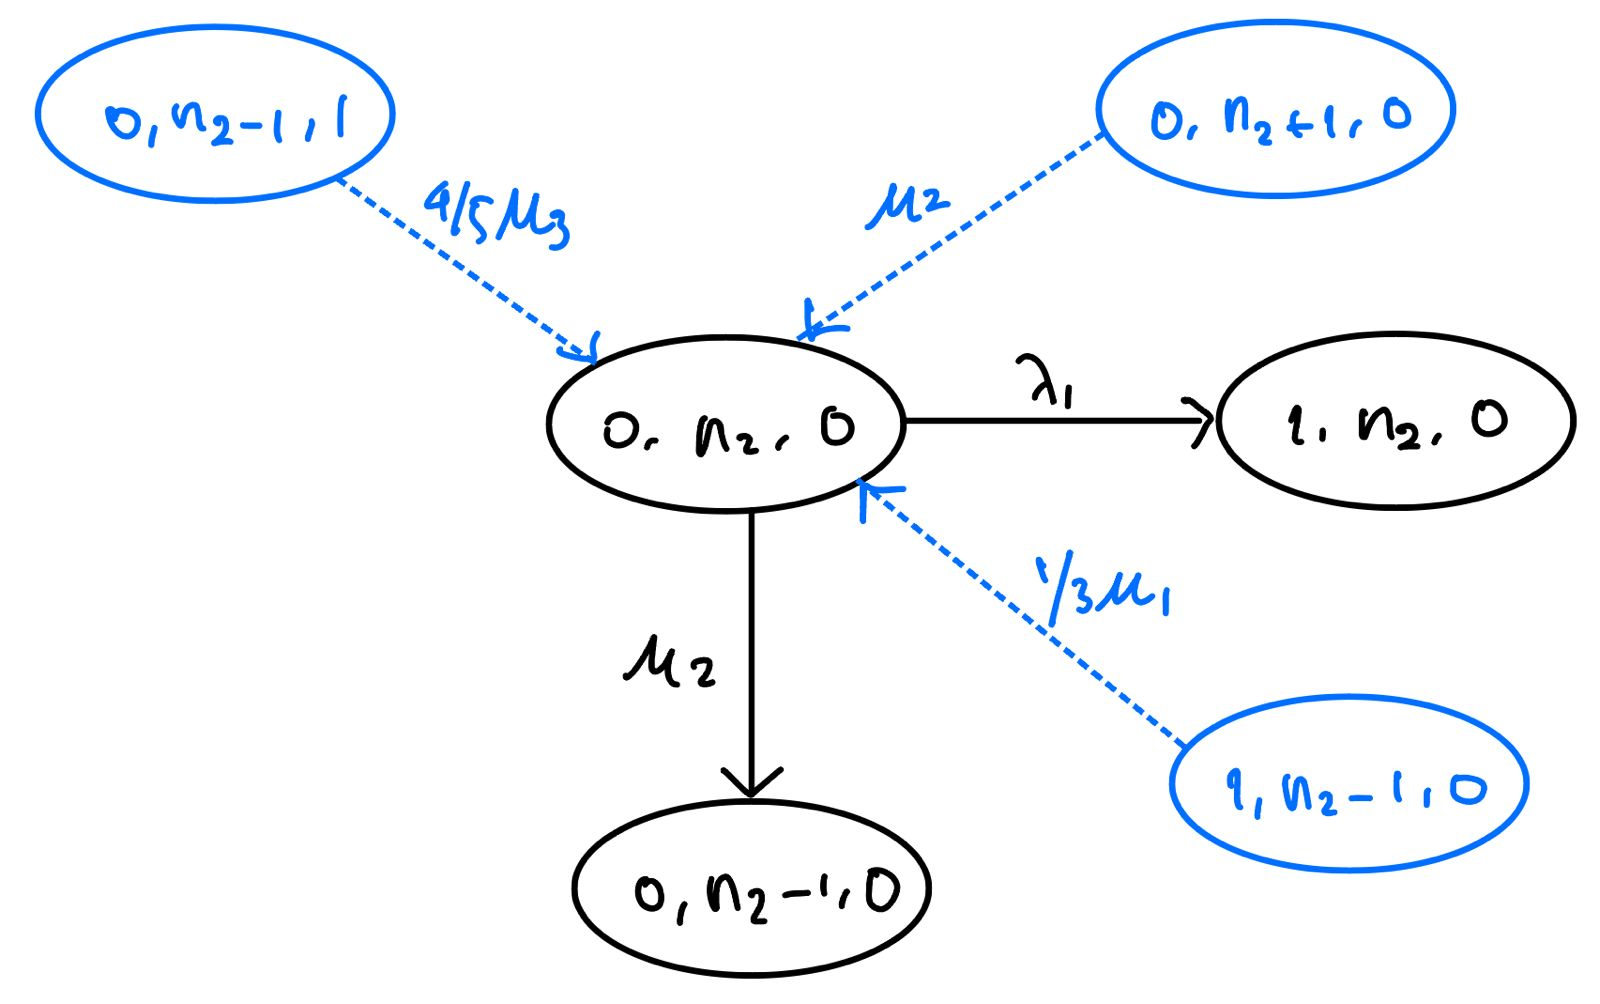
\includegraphics[width=0.7\linewidth]{0,n2,0.jpg}
        \caption{$0,n_2,0$}
        \label{fig:enter-label1}
    \end{figure}
\end{frame}

\begin{frame}{Diagram Transition}
    \begin{figure}
        \centering
        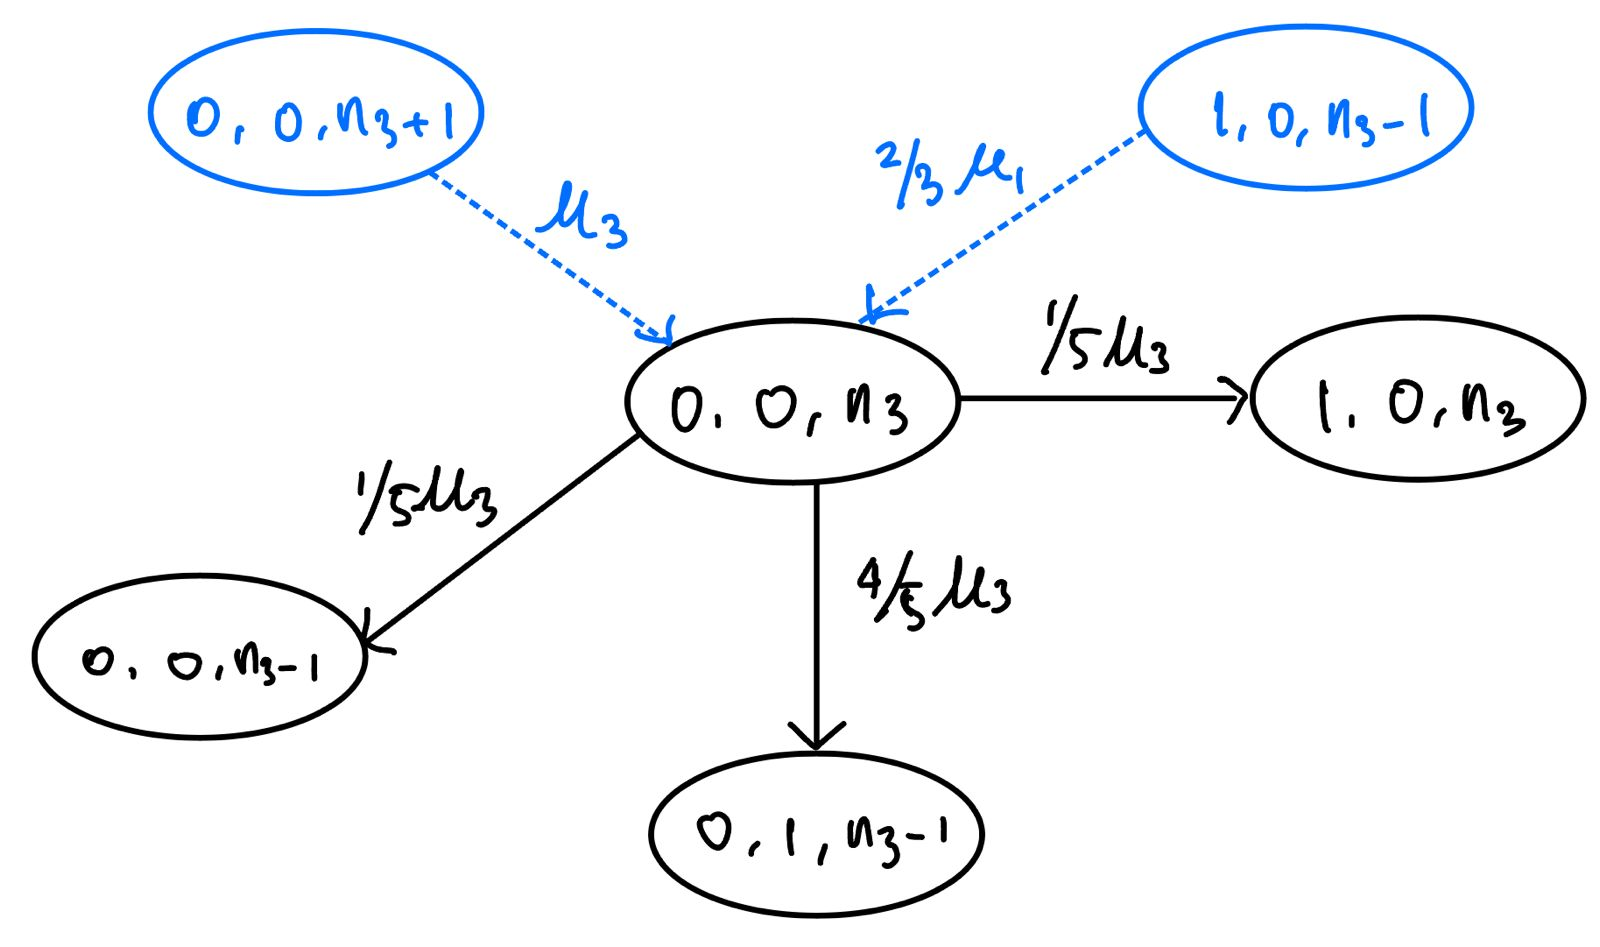
\includegraphics[width=0.7\linewidth]{0,0,n3.jpg}
        \caption{$0,0,n_{3}$}
        \label{fig:enter-label1}
    \end{figure}
\end{frame}

\begin{frame}{Diagram Transition}
    \begin{figure}
        \centering
        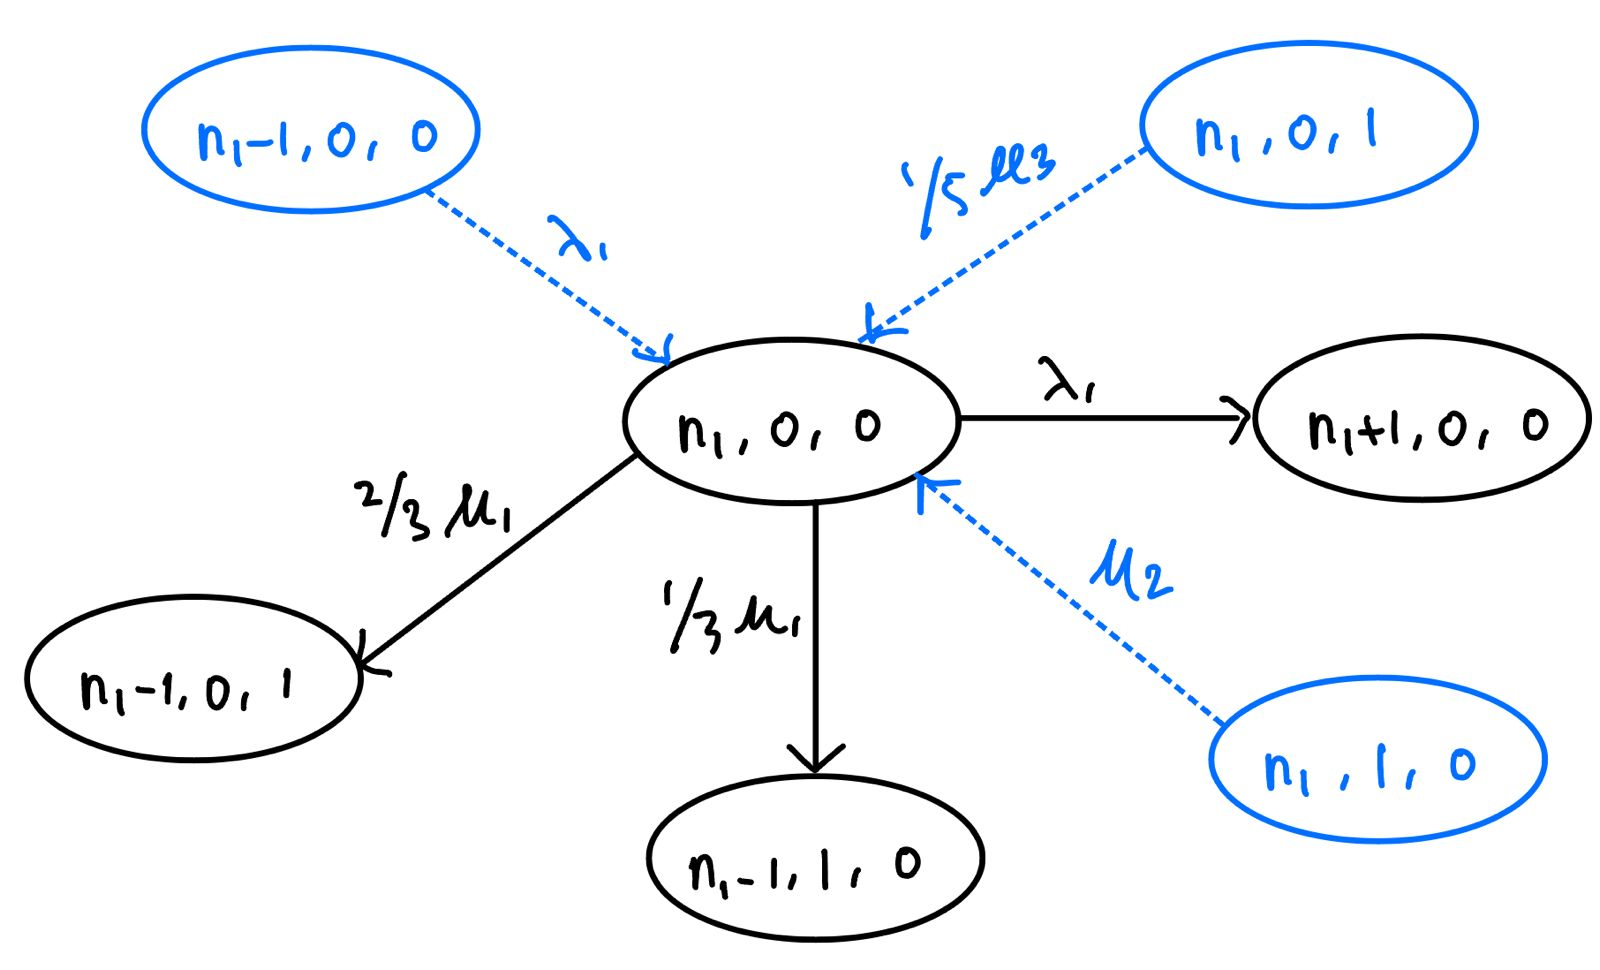
\includegraphics[width=0.7\linewidth]{n1, 0, 0.jpg}
        \caption{$n1,0,0$}
        \label{fig:enter-label1}
    \end{figure}
\end{frame}

\begin{frame}{Diagram Transition}
    \begin{figure}
        \centering
        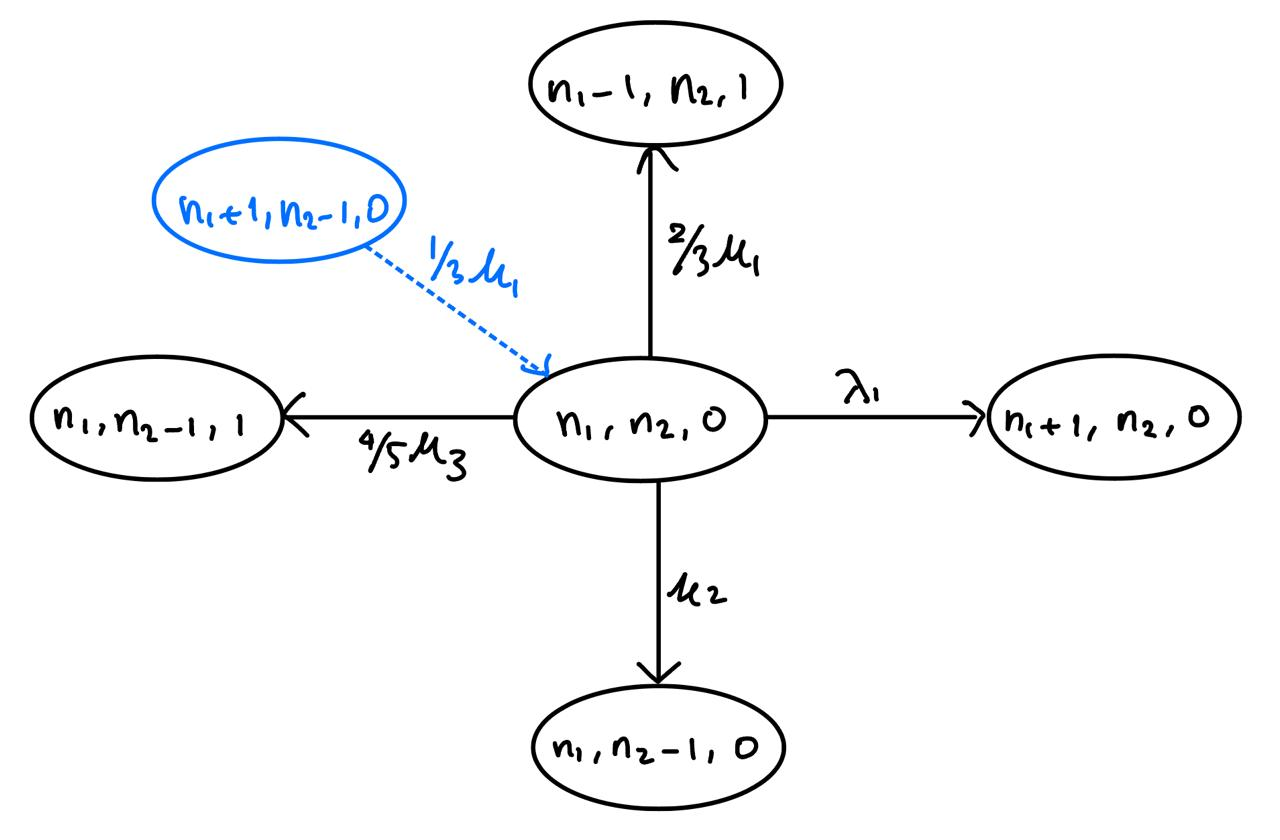
\includegraphics[width=0.7\linewidth]{n1,n2,0.jpg}
        \caption{$n_1,n_2,0$}
        \label{fig:enter-label1}
    \end{figure}
\end{frame}

\begin{frame}{Diagram Transition}
    \begin{figure}
        \centering
        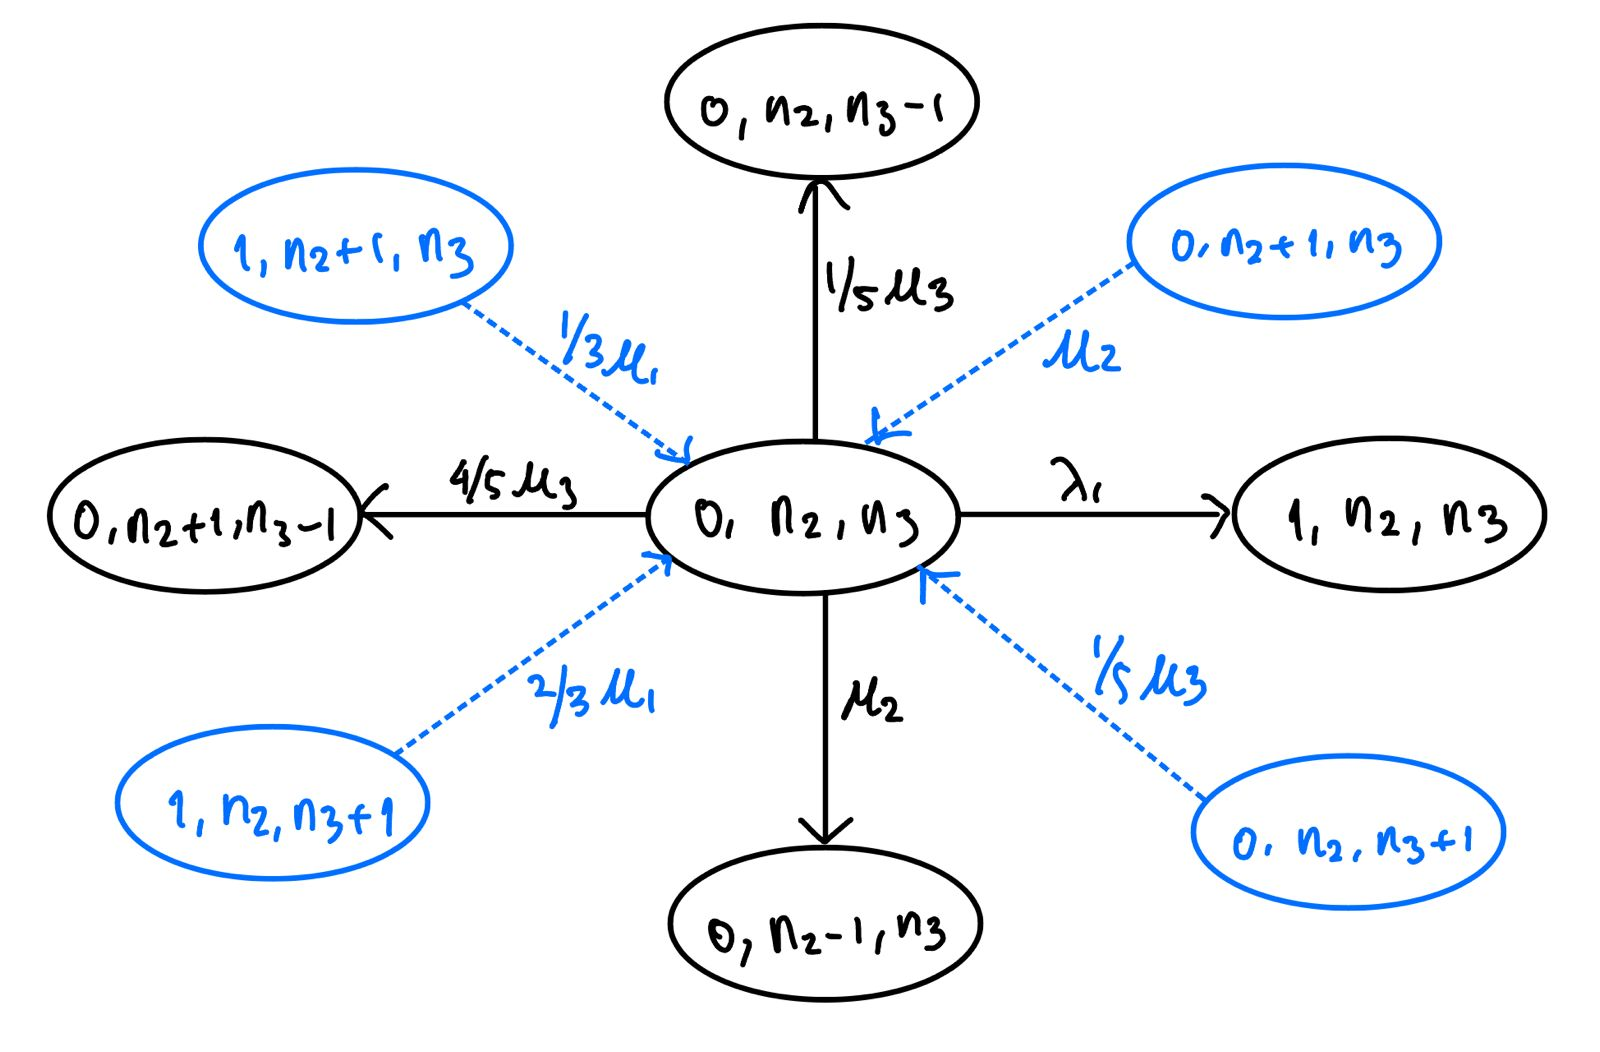
\includegraphics[width=0.7\linewidth]{0,n2,n3.jpg}
        \caption{$0,n_2,n_{3}$}
        \label{fig:enter-label1}
    \end{figure}
\end{frame}

\begin{frame}{Diagram Transition}
    \begin{figure}
        \centering
        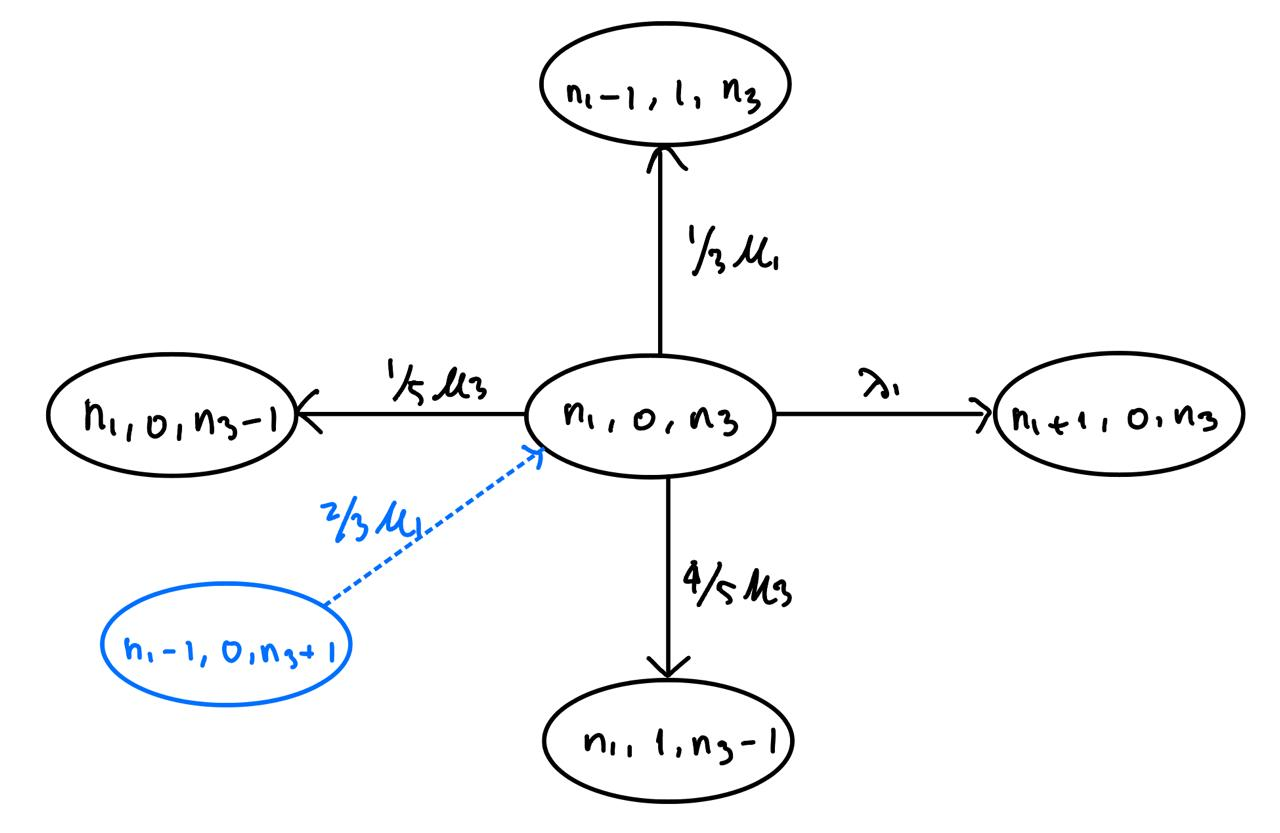
\includegraphics[width=0.7\linewidth]{n1, 0, n3.jpg}
        \caption{$n_1,0,n_{3}$}
        \label{fig:enter-label1}
    \end{figure}
\end{frame}





\section{\color{mygreen}\huge Balance equations}
\begin{frame}{Balance Equations}
    \begin{enumerate}
        \item Kasus $n_{1}=n_{2}=n_{3}=0$\
        $$\lambda_{1}P_{000}=\frac{1}{3}\mu_{1}P_{010}+\frac{2}{3}\mu_{1}P_{001}$$
        \item Kasus $n_{1}> 0 , n_{2}=n_{3}=0$\
        $$(\mu_1 + \lambda_1)P_{n_1, 0, 0} + \frac{1}{5}\mu_3 P_{n_1, 0, 1} + \mu_2 P_{n_1, 1, 0}$$
        \item Kasus $n_{1}=0, n_{2}>0 , n_{3}=0$\   $$[\lambda_{1}+\mu_{1}]P_{0,n_{2},0}=\frac{1}{3}\mu_{1}P_{1,n_{2}-1,0}+\mu_{2}P_{0,n_{2}+1,0}+\frac{4}{5}\mu P_{0,n_{2}-1,1}$$
        \item Kasus $n_{1}=n_{2}=0 , n_{3}>0$\
        $$[\frac{1}{5}\mu_{3}+\frac{4}{5}\mu_{3}+\lambda_{1}]P_{0,0,n_{3}}=\frac{2}{3}\mu_{1}P_{1,0,n_{3}-1}+\mu_{3}P_{0,0,n_{3}+1}$$
        
\end{enumerate}
\end{frame}
    \begin{frame}{Balance Equations}
    \begin{enumerate}
        \item [5.] Kasus $n_{1}>0 , n_{2} > 0, n_{3} > 0$\\
        $[\lambda_{1}+\mu_{1}+\mu_{2}+\mu_{3}]P_{n_{1},n_{2},n_{3}}=\lambda_{1}P_{n_{1}-1,n_{2},n_{3}}+\frac{1}{3}\mu_{1}P_{n_{1}+1,n_{2}-1,n_{3}}+\frac{2}{3}\mu_{1}P_{n_{1}+1,n_{2},n_{3}-1}+\mu_{2}P_{n_{1},n_{2}+1,n_{3}}+\frac{1}{5}\mu_{3}P_{n_{1},n_{2},n_{3}+1}+\frac{4}{5}\mu_{3}P_{n_{1},n_{2}-1,n_{3}+1}$
        \item [6.] Kasus $n_{1}>0 , n_{2}>0 , n_{3}=0$
        $$(\frac{2}{3}\mu_1 + \lambda_1 + \mu_2)P_{n_1, n_2, 0} = \frac{1}{3} \mu_1 P_{n_1 +1, n_2 -1, 0} + \frac{4}{5}\mu_3 P_{n_1, n_2 - 1, 1}$$
        \item [7.] Kasus $n_{1}=0 , n_{2}>0 , n_{3}>0$
        $$(\mu_3 + \mu_2 + \lambda_1)P_{0, n_2, n_3} = \frac{2}{3}P_{1, n_2, n_3 + 1} + \frac{1}{5}P_{0, n_2, n_3 + 1} + \mu_2 P_{0, n_2 + 1, n_3} + \frac{1}{3} \mu_1 P_{1, n_2 + 1, n_3}$$
        \item [8.] Kasus $n_{1}>0, n_{2}=0, n_{3}>0$
        $$(\frac{1}{3}\mu_1 + \mu_3 + \lambda_1)P_{n_1, 0, n_3} = \frac{2}{3}\mu_1 P_{n_1 - 1, 0, n_3 + 1}$$
    \end{enumerate}
    \end{frame}
        


%\begin{frame}{Pembahasan}
 %   \begin{rbox}{Penurunan Model Jaringan Antrean Open Jackson pada Rumah Sakit (Lanjutan)}
       % Selanjutnya, akan dicari $P_{ij}$ dengan mengubah terlebih dahulu bentuk sistem \textit{Balance Equations} sebelumnya ke bentuk matriks, yaitu:
      %  \begin{figure}
          %  \centering
            %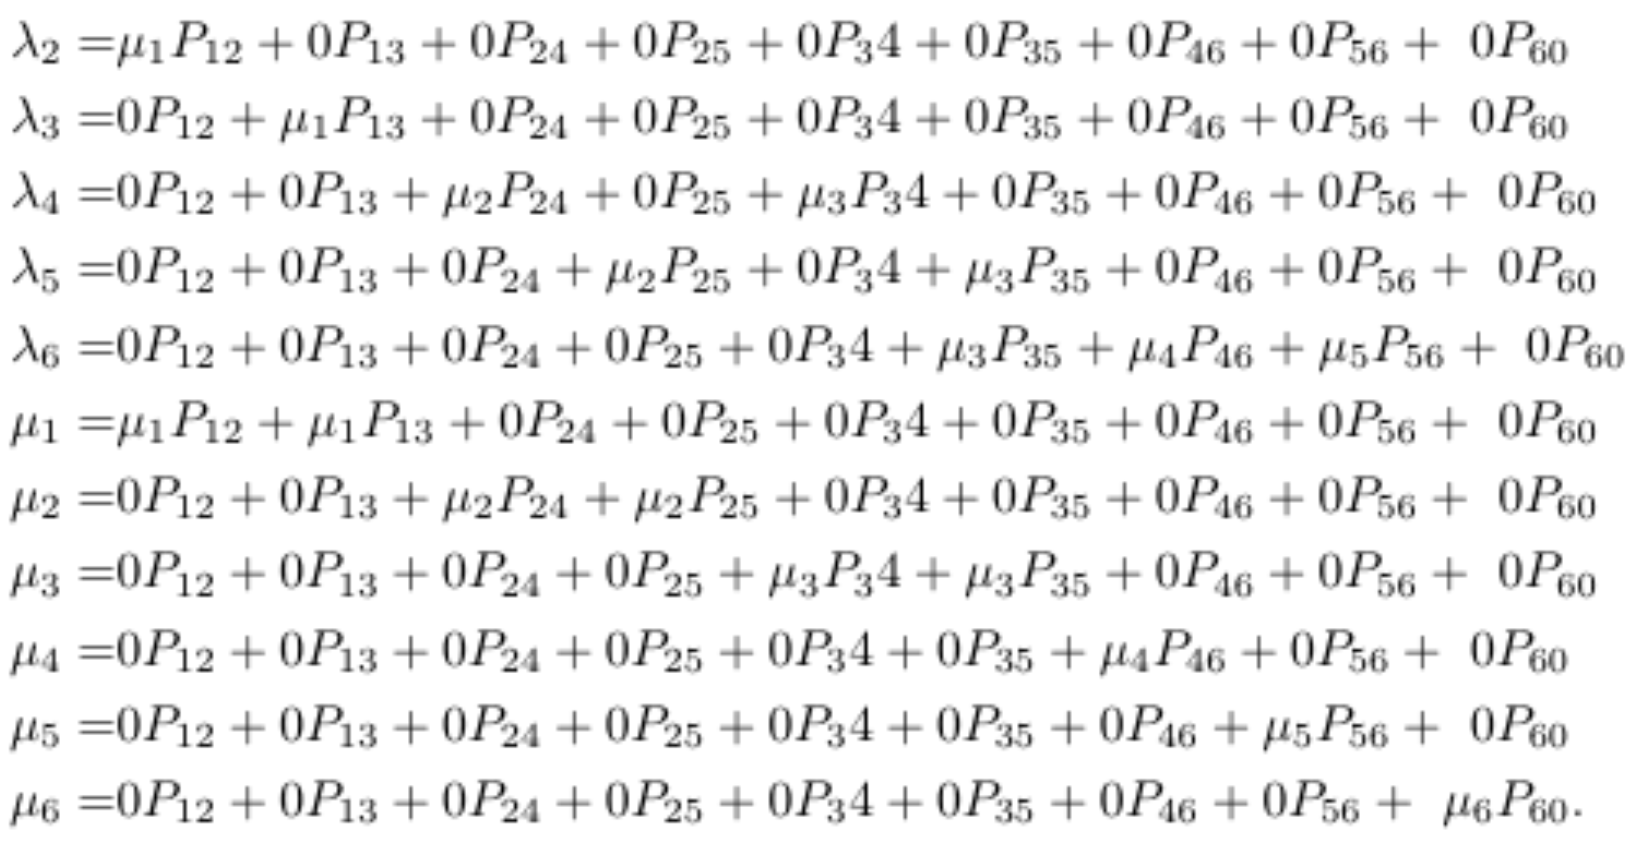
\includegraphics[width=0.5\linewidth]{Images/Balance Eqs.png}
           % \caption{Persamaan Balance}
           % \label{fig:enter-label}
       % \end{figure}
    %\end{rbox}
    
%\end{frame}

     

\section{\color{mygreen}\huge Kesimpulan}
\begin{frame}{Kesimpulan}
 
  %  Berdasarkan hasil pembahasan, sistem antrian di enam stasiun layanan, dapat disimpulkan bahwa masing-masing stasiun layanan mengikuti model (M/M/1): (FCFS/∞/∞). Hasil pembahasan diperoleh nilai probabilitas transisi antar stasiun. Probabilitas transisi dari stasiun 1 ke stasiun 2 dan 3, dari stasiun 2 ke stasiun 4 dan 5, dari stasiun 3 ke Stasiun 4 dan 5 dan dari stasiun 4 ke stasiun 6 berturut-turut adalah 0,4436053 dan 0,5563947, 0.5153421 dan 0,4846579, 0.5159005 dan 0.4840995, 0,9461371 dan 0,9185853 masing-masing. Probabilitas transisi pasien keluar dari sistem dari stasiun 6 adalah 1.0000004.
%Selain itu, jumlah rata-rata pasien di sistem antrian di semua stasiun layanan adalah 39 pasien, sementara waktu tunggu rata-ratanya pasien di sistem antrian adalah 54.6101 menit. 
\end{frame}

\begin{frame}
	
	\begin{tikzpicture}[overlay, remember picture]
		\node[xshift=5cm,yshift=-5.32cm]{
\includegraphics[width=12cm]{img1}
		};
	\end{tikzpicture}

	\begin{tikzpicture}[overlay, remember picture]
		\node[xshift=4.1cm,yshift=0mm]{
\includegraphics[width=7cm]{Ty}
		};
	\end{tikzpicture}

	\hspace{8 cm}\textit{\color{mygreen}\huge Terima {\color{mygreen!50}Kasih}}
\end{frame}

\end{document}

